\documentclass[sigconf]{acmart}

\usepackage{balance}	% balancing bibstyles as per request in accepted submission


%% These commands are for a PROCEEDINGS abstract or paper.
\copyrightyear{2021}
\acmYear{2021}
\setcopyright{acmcopyright}
\acmConference[ACM-BCB '21]{ACM-BCB '21: ACM Conference on Bioinformatics, Computational Biology, and Health Informatics}{August 01--04, 2021}{Online}
\acmBooktitle{}
\acmPrice{}
\acmISBN{}
\acmDOI{}

	\author{Halie M. Rando}
			\orcid{0000-0001-7688-1770}
				\affiliation{
							\institution{University of Pennsylvania}
										\department{Department of Systems Pharmacology and Translational Therapeutics}
										\city{Philadelphia}
										\state{PA}
										\country{USA}
					}
			\affiliation{
							\institution{University of Colorado School of Medicine}
										\department{Department of Biochemistry and Molecular Genetics}
														}
			\affiliation{
										\department{Center for Health AI}
										\city{Aurora}
										\state{CO}
										\country{USA}
					}
				\email{halie.rando@cuanschutz.edu}
		\author{Simina M. Boca}
			\orcid{0000-0002-1400-3398}
				\affiliation{
							\institution{Georgetown University Medical Center}
										\department{Innovation Center for Biomedical Informatics}
										\city{Washington}
										\state{DC}
										\country{USA}
					}
				\email{smb310@georgetown.edu}
		\author{Lucy D'Agostino McGowan}
			\orcid{0000-0001-7297-9359}
				\affiliation{
							\institution{Wake Forest University}
										\department{Department of Mathematics and Statistics}
										\city{Winston-Salem}
										\state{NC}
										\country{USA}
					}
				\email{lucydagostino@gmail.com}
		\author{Daniel S. Himmelstein}
			\orcid{0000-0002-3012-7446}
				\affiliation{
							\institution{None}
																	}
				\email{daniel.himmelstein@gmail.com}
		\author{Michael P. Robson}
			\orcid{0000-0002-4859-0033}
				\affiliation{
							\institution{Villanova University}
										\department{Department of Computing Sciences}
										\city{Villanova}
										\state{PA}
										\country{USA}
					}
				\email{michael.robson@villanova.edu}
		\author{Vincent Rubinetti}
			\orcid{0000-0002-4655-3773}
				\affiliation{
							\institution{University of Pennsylvania}
										\department{Perelman School of Medicine}
										\city{Philadelphia}
										\state{PA}
										\country{USA}
					}
			\affiliation{
							\institution{University of Colorado School of Medicine}
										\department{Center for Health AI}
										\city{Aurora}
										\state{CO}
										\country{USA}
					}
				\email{vince.rubinetti@gmail.com}
		\author{Ryan Velazquez}
			\orcid{0000-0002-3655-3403}
				\affiliation{
							\institution{Azimuth1}
													\city{McLean}
										\state{VA}
										\country{USA}
					}
				\email{rnhvelazquez@gmail.com}
		\author{COVID-19 Review Consortium}
				\affiliation{
							\institution{None}
																	}
			\author{Casey S. Greene}
			\orcid{0000-0001-8713-9213}
				\affiliation{
							\institution{University of Pennsylvania}
										\department{Department of Systems Pharmacology and Translational Therapeutics}
														}
			\affiliation{
							\institution{Alex's Lemonade Stand Foundation}
										\department{Childhood Cancer Data Lab}
										\city{Philadelphia}
										\state{PA}
										\country{USA}
					}
			\affiliation{
							\institution{University of Colorado School of Medicine}
										\department{Department of Biochemistry and Molecular Genetics}
														}
			\affiliation{
										\department{Center for Health AI}
										\city{Aurora}
										\state{CO}
										\country{USA}
					}
				\email{greenescientist@gmail.com}
		\author{Anthony Gitter}
			\orcid{0000-0002-5324-9833}
				\affiliation{
							\institution{University of Wisconsin-Madison}
										\department{Department of Biostatistics and Medical Informatics}
														}
			\affiliation{
							\institution{Morgridge Institute for Research}
													\city{Madison}
										\state{WI}
										\country{USA}
					}
				\email{gitter@biostat.wisc.edu}
	

\begin{document}


	\title{An Open-Publishing Response to the COVID-19 Infodemic}




\renewcommand{\shortauthors}{}


\maketitle
\bibliographystyle{ACM-Reference-Format}

	{\let\thefootnote\relax\footnote{Conflicts of interest. Lucy D'Agostino McGowan: Received consulting fees from Acelity and Sanofi in the past five years. Anthony Gitter: Filed a patent application with the Wisconsin Alumni Research Foundation related to classifying activated T cells.}}

\hypertarget{abstract}{%
\section{ABSTRACT}\label{abstract}}

The COVID-19 pandemic catalyzed the rapid dissemination of papers and preprints related to the disease.
The multifaceted nature of COVID-19 demands a multidisciplinary approach, but the urgency of the crisis combined with the need for social distancing measures presents unique challenges to collaborative science.
We sought to apply a massive online open publishing approach to this problem using Manubot.
Through GitHub, collaborators contributed summaries and critiques of literature via issue templates and contributed literature summaries as pull requests.
Manubot rendered the manuscript content into pdf, HTML, and docx outputs, and an up-to-date version was always available online.

This particular project presented unique challenges that necessitated additions to Manubot.
Some challenges related to the technical barrier to entry, as most contributors were from biomedical backgrounds and had limited experience with git.
We developed training resources to allow participation through GitHub's web interface and added support for the citation of clinical trial identifiers and spell-checking.
We also expanded the range of formats and options available for export.
The other category of challenges arose because of the extreme volume and velocity of COVID-19 publications.
We adapted Manubot's figure generation workflow to retrieve up-to-date data from online sources nightly.
Additionally, we integrated scite, a tool for checking the status of references, including retractions, into the HTML build to simplify the process of monitoring changes to publications after their release.

Through this effort, we organized over 50 scientists from a range of backgrounds who evaluated over 1000 sources and authored seven literature reviews.
This project illustrates that Manubot is an adaptable workflow that can handle even an extreme volume and velocity of information and that its back-end technical complexity does not prohibit the inclusion of non-technical contributors.
While many efforts from the computational community have focused on mining COVID-19 literature, this implementation illustrates the power of open publishing to organize people to aggregate and disseminate information in response to an evolving crisis.
Applying this approach allowed us to develop a community that occupies a unique niche in the COVID-19 research space.

\hypertarget{ccs-concepts}{%
\section{CCS CONCEPTS}\label{ccs-concepts}}

\hypertarget{keywords}{%
\section{KEYWORDS}\label{keywords}}

COVID-19, open publishing, open-source, data integration, manubot

\hypertarget{introduction}{%
\section{INTRODUCTION}\label{introduction}}

Coronavirus Disease 2019 (COVID-19) has shaped the years 2020 and 2021 by causing a worldwide public health crisis.
The scientific community has responded by turning significant attention and resources towards COVID-19 and the associated virus, SARS-CoV-2.
The result has been the rapid release of data, results, and publications related to COVID-19 at a scale never previously seen.
Over 20,000 articles about COVID-19 were released in the first four months of the pandemic \citep{7ub6VM4Z}, and the velocity and volume of information being released led to the pandemic being termed an ``infodemic'' as well \citep{7ub6VM4Z, nnfOazAC}.
While this influx of information is likely evidence of important work towards understanding the virus and the disease, there are also downsides to the availability of too much information.
The downsides of ``excessive publication'' have been recognized for over forty years, as it was raised as a major concern about the move towards electronic, rather than print, publishing at the turn of the millennium \citep{DfSr1Ohc}.
The contents of the COVID-19 Open Research Dataset (CORD-19) \citep{CiOwklc6}, which was developed in part to assist in efforts to train machine learning algorithms on COVID-19-related text, illustrates the volume of publication relevant to understanding this virus (Figure \ref{fig:cord19-growth}).
This resource was developed by querying several sources for terms related to SARS-CoV-2 and COVID-19, as well as the coronaviruses SARS-CoV-1 and MERS-CoV and their associated viruses \citep{CiOwklc6} and contained 552928 manuscripts as of 2021-05-03.
Additional curation by CoronaCentral \citep{zQ1JIn2J} has produced, at present, a set of over 150,000 publications particularly relevant to COVID-19 and these closely related viruses.
Thus, any effort to synthesize, summarize, and contextualize COVID-19 research will face a vast corpus of potentially relevant material.

\textbf{Change over time in the number of publications in the CORD-19 dataset.}
As of 2021-05-03, there were 552928 articles in the CORD-19 dataset.
The first release, on March 16, 2020, contained 28,000 manuscripts on topics relevant to SARS-CoV-2 and related coronaviruses \citep{CiOwklc6}.
Since then, these articles have continued to proliferate (left), with both traditionally published and preprint manuscripts in the corpus (right).
At present, it contains 24304 preprints from \emph{arXiv}, \emph{bioRxiv}, and \emph{medRxiv}.
While not all of the manuscripts are focused explicitly on SARS-CoV-2 or COVID-19, this corpus is likely to contain all or most manuscripts relevant to writing a literature review, which requires assessing both emerging and prior research.
{]}(https://github.com/greenelab/covid19-review/raw/e35e528aa516fc6177c057ee4c952cb6fc52cc5a/CORD-19/cord19-growth.png ``CORD-19 dataset growth'')\{\#fig:cord19-growth secno=1\}

With information being produced rapidly through both traditional publishing venues and preprint servers, some papers that are published face scrutiny after their initial release.
Concerns have been raised that the number of COVID-19 papers being retracted may be higher, or potentially much higher, than is typical, although a thorough investigation of this question will not be possible until more time has elapsed \citep{ZUk10707, caxpZEmy}.
Other papers are updated with corrections or expressions of concern {[}\citet{caxpZEmy};url:https://retractionwatch.com/retracted-coronavirus-covid-19-papers{]}.
These include both preprints and papers published in more traditional venues \citep{hfAF6aDr, paRLhIdE}.
Preprints provide a venue for scientists to release findings rapidly but have both the advantage and disadvantage of making research available before it has undergone the peer-review process.
However, some traditional publishing venues have also fast-tracked COVID-19 through peer review, leading to questions about whether this research is being held to the usual standards for publication \citep{1Dez1ZOc5}.
Therefore, monitoring the COVID-19 literature requires not only digesting the high volume of information released but also critically evaluating it and/or monitoring for subsequent adjustments.

Because of the fast-moving nature of the topic, many efforts to summarize and synthesize the COVID-19 literature have been undertaken.
These efforts include newsletters \citetext{\citealp{d204tUzq}; \citealp{JdWiPJCL}}, web portals (such as \citep{m4B8roc9, 1CBWvhTdy} or the now-defunct http://covidpreprints.com/, which was described in \citep{paRLhIdE}), comments on preprint servers \citep{YZ4cHNuH} (see https://disqus.com/by/sinaiimmunologyreviewproject), and even a journal \citep{oBoqEGzZ}.
However, the explosive rate of publication presents challenges for such efforts, many of which are no longer publishing summaries.
Similarly, many literature reviews have been written on the available COVID-19 literature \citep{I2EsJmfs, 5x25saIz, evtsR3C5, 5x25saIz, 18eCxyLhx, SAE5ME3N, xOs5ctsW}.
However, static reviews quickly become outdated as new research is released or existing research is retracted or superseded; one example is a review of topics in COVID-19 research including vaccine development \citep{xOs5ctsW}.
This review was published on July 10, 2020, four days before Moderna released the surprisingly promising results of their phase 1 trial \citep{wiGjCZC8} that changed expectations surrounding vaccines.
Therefore, the COVID-19 publishing climate presented a challenge where curation of the literature by a diverse group of experts in a format that could respond quickly to high-volume, high-velocity information was desirable.

We therefore sought to develop a platform for scientific discussion and collaboration around COVID-19 by adapting open publishing infrastructure to accommodate the scale of the COVID-19 publishing boom.
Recent advances in open publishing have created an infrastructure that facilitates distributed, version-controlled collaboration on manuscripts \citep{YuJbg3zO}.
Manubot \citep{YuJbg3zO} is a collaborative framework developed to adapt open-source software development techniques and version control for manuscript writing.
With Manubot, manuscripts are managed and maintained using GitHub, a popular, online version control interface.
This open-publishing platform has been used to develop large-scale collaborative efforts such as a review of developments in deep learning \citep{PZMP42Ak} and a re-evaluation of the role of authorship in modern collaborations \citep{6acsZuy7}.
Collaboration via massively open online papers has been identified as a strategy for promoting inclusion and interdisciplinary thought \citep{PoDz2q0A}.
Manubot is an ideal platform for analyzing COVID-19 literature because it facilitates the automatic integration of new data through CI.
However, the Manubot workflow can appear intimidating to contributors who are not well-versed in git \citep{PoDz2q0A}.
The synthesis and discussion of the emerging literature by biomedical scientists and clinicians is imperative to a robust interpretation of COVID-19 research, but in biology, such efforts often rely on What You See Is What You Get tools such as Google Docs, despite the significant limitations of these platforms in the face of excessive publication.
Therefore, we recognized that the problem of synthesizing the COVID-19 literature lent itself well to the Manubot platform, but that the potential technical expertise required to work with Manubot present a significant technical barrier to domain experts.

Here, we describe efforts to adapt Manubot to handle the extreme case of the COVID-19 infodemic, with the objective of extending manuscript reviewing to develop a centralized platform for summarizing and synthesizing a massive amount of preprints, news stories, journal publications, and data.
Unlike prior collaborations built on Manubot, here most contributors came from a traditional biological or medical background.
The members of the COVID-19 Review Consortium worked to consolidate information about the virus in the context of related viruses and to synthesize rapidly emerging literature centered on the diagnosis and treatment of COVID-19.
Manubot provided the infrastructure to manage contributions from the community and create a living, scholarly document that integrated data from multiple sources to respond to the COVID-19 crisis in real time and a back-end that allowed biomedical scientists to sort and distill informative content out of the overwhelming flood of information \citep{1HZeeO4Cs}, in order to provide a resource that would be useful to the broader scientific community.
This case study demonstrates the value of open collaborative writing tools such as Manubot to emerging challenges and the flexibility of Manubot to be adapted to problems unique to a range of fields.
By recording the evolution of information over time and assembling a resource that auto-updated in response to the evolving crisis, it revealed the particular value that Manubot holds for managing rapid changes in scientific thought.

\hypertarget{methods}{%
\section{METHODS}\label{methods}}

\hypertarget{contributor-recruitment-and-roles}{%
\subsection{Contributor Recruitment and Roles}\label{contributor-recruitment-and-roles}}

A preliminary requirement for this undertaking was to establish Manubot as a platform accessible to researchers with limited experience working with git, as is common in biology and medicine, where version control is not typically emphasized \citep{1HmO21gZN, OO1DuZd, 4ny1onB0}.
Contributors were recruited by word of mouth and on Twitter, and we sought out opportunities to integrate existing efforts to train early-career researchers (ECRs).
We invited potential collaborators to contribute a short introduction on a GitHub issue in order to collect information about who was involved and provide an introduction to working with GitHub issues.
Interested participants were encouraged to contribute in several ways.
One option was to catalog articles of interest as issues in the GitHub repository.
We developed a standardized set of questions for contributors to consider when evaluating an article following a framework often used for assessing medical literature.
This approach emphasizes examining the methods used, assignment (whether the study was observational or randomized), assessment, results, interpretation, and how well the study extrapolates \citep{17OQtAY4l}.
Contributors were also invited to contribute or edit text using GitHub's pull request system.
These contributions were not strictly defined and could range from minor corrections to punctuation and grammar to large-scale additions of text.
Each pull request was reviewed and approved by at least one other contributor before being merged into the main branch.
We sought to tag potential reviewers based on the introductions they had contributed in order to encourage participation.
Emphasizing the use of issues and pull requests was designed to encourage authors with and without git experience to discuss papers and provide feedback (both formal and informal) on proposed text additions or changes.
We also used gitter (\citet{iXfPU3Cy}) to promote informal questions and sharing of information among collaborators.

\hypertarget{utilization-and-expansion-of-manubot}{%
\subsection{Utilization and Expansion of Manubot}\label{utilization-and-expansion-of-manubot}}

Applying Manubot's existing capabilities allowed us to confront several challenges common in large-scale collaborations, such as maintaining a record of contributions that allowed us to allocate credit appropriately or to contact the original author if questions arose.
Additionally, an up-to-date version of the content was available at all times online at https://greenelab.github.io/covid19-review/.
This approach also allowed us to minimize the demand on authors to curate bibliographic resources.
Manubot provides the functionality to create a bibliography using digital object identifiers (DOIs), website URLs, or other identifiers such as PubMed identifiers and arXiv IDs.
The author can insert a citation in-line using a format such as \texttt{{[}@doi:10.1371/journal.pcbi.1007128{]}}.
Manubot then obtains reference metadata, exports the citations as Citation Style Language JSON Data Items, which is an open standard, and renders the bibliographic information needed to generate the references section \citep{YuJbg3zO}.
This approach allows multiple authors to work on a piece of text without needing to make manual adjustments to the reference lists.

Due to the needs of this project, several new features were also implemented in Manubot.
Because of the ever-evolving nature of the COVID-19 crisis, many of the figures and text proposed by subject matter contributors would have quickly become outdated.
To address this concern, Manubot and GitHub's CI features were used to create figures that integrated online data sources to respond to changes in the COVID-19 pandemic over time.
The combination of Manubot and GitHub Actions also made it possible to dynamically update information, such as the current number of active COVID-19 clinical trials \citep{cifK9B8t}, within the text of the manuscripts.
GitHub Actions runs a nightly workflow to update these external data and regenerate the statistics and figures for the manuscript.
The workflow uses the GitHub API to detect and save the latest commit of the external data sources, which are both GitHub repositories.
It then downloads versioned data from that snapshot of the external repositories and runs bash and Python scripts to calculate the desired statistics and produce the summary figures.
The statistics are stored in JSON files that are accessed by Manubot to populate the values of placeholder template variables dynamically every time the manuscript is built.
For instance, the template variable \texttt{\{\{ebm\_trials\_results\}\}} in the manuscript is replaced by the actual number of clinical trials with results, 98.
The template variables also include versioned URLs to the dynamically updated figures.
The JSON files and figures are stored in the \texttt{external-resources} branch of the manuscript's GitHub repository, which acts as versioned storage.
The GitHub Actions workflow automatically adds and commits the new JSON files and figures to the \texttt{external-resources} branch every time it runs, and Manubot uses the latest version of these resources when it builds the manuscript.
For figures, data are then plotted using Matplotlib \citep{1026Gxdsi} in Python and pushed to a branch where they can be read into the main manuscript.
The workflow file is available from \url{https://github.com/greenelab/covid19-review/blob/master/.github/workflows/update-external-resources.yaml}, and the scripts are available from \url{https://github.com/greenelab/covid19-review/tree/external-resources}.
The Python package versions are available in \url{https://github.com/greenelab/covid19-review/blob/external-resources/environment.yml}.

Another issue that emerged was the need for a standardized way to cite clinical trials.
Clinical trials that are registered with https://clinicaltrials.gov receive a unique clinical trial identifier, or ``NCT ID.''
Because clinical trials are registered long before results are available in manuscript form, it was important to this project to be able to refer to the clinical trial identifiers associated with a large number of relevant trials (Figure \ref{fig:ebm-trials}).
Manubot uses the Zotero translation server (https://www.zotero.org and https://github.com/zotero/translation-server) to extract metadata for some types of citations.
However, Zotero did not support clinical trial identifiers and could not extract relevant metadata from the clinical trial's URL.
In order to enable Manubot to pull metadata associated with clinical trials based on their identifiers, we added Zotero support for these identifiers.
Other researchers identified the same need \citep{ZQPtEdnO, thdq2nGf}.
To implement this feature, we query clinicaltrials.gov to retrieve XML metadata associated with each identifier using JavaScript \citep{Bxfd7L4s}.
Then, when Manubot requests clinical trial metadata from the Zotero translation server, it receives a more informative response that includes the trial sponsors, responsible investigators, title, and summary.
We extended Manubot to support directly citing any of the hundreds of Compact Uniform Resource Identifier registered with \url{https://identifiers.org/}, including the \texttt{clinicaltrials} identifier.
This extension enables citing a trial as \texttt{clinicaltrials:NCT04280705} instead of \texttt{https://clinicaltrials.gov/ct2/show/NCT04280705}.

Another challenge that emerged was that, because of the large number of citations used in this manuscript and the fast-moving nature of COVID-19 research, keeping track of retractions, corrections, and notices of concern became a priority.
We implemented a new Manubot plugin to support ``smart citations'' in the HTML build of manuscripts.
The plugin uses the \href{https://scite.ai/}{Scite} \citep{14UJbLWf4} service to display a badge below any citation with a DOI.
The badge contains a set of icons and numbers that indicate how many times that source has been mentioned, supported, or disputed and whether there have been any important editorial notices, such as retractions or corrections.
Using this, we were able to identify references that needed to be reevaluated.
This addition was invaluable given the nature of the project, where we were disseminating rapidly evolving information of great consequence from over a thousand different sources.
The badges also allow readers to ascertain a rough evaluation of the reliability of cited sources at a glance.

Because most collaborators were writing and editing text through the GitHub website rather than in a local text editor, we also needed to add spell-checking functionalities to Manubot.
We integrated an existing Pandoc (https://pandoc.org/) spell-check extension with AppVeyor CI to automatically post spelling errors as comments in a GitHub pull request.
The comment reported both unique misspelled words and all locations in which those spelling errors were detected.
Project maintainers created and updated a custom dictionary to ignore over 1,500 scientific and technical terms that are not common English words.
Spell-checking also helped standardize the writing style across dozesn of authors by detecting British English spelling.
The actual spell-checking was implemented using GNU Aspell (http://aspell.net/) and the Pandoc spellcheck filter \citep{nTjoZqSQ}.
The filter enables checking only the manuscript text, ignoring URLs and formatting text.

Manubot can render a manuscript in several formats that serve different purposes.
Prior to this project, Manubot was able to convert the markdown-formatted manuscript to HTML, pdf, and docx formats.
For the current project, we expanded this functionality to allow for individual sections of the manuscript to be rendered as separate docx files.
This development was necessary because our initial manuscript grew so large that it needed to be split into seven separate papers for submission.
Similarly, we expanded the range of possible export formats to include LaTeX.
This automation was desirable because LaTeX is used for manuscript submission in many fields.

\hypertarget{results}{%
\section{RESULTS}\label{results}}

\hypertarget{recruitment-and-manuscript-development}{%
\subsection{Recruitment and Manuscript Development}\label{recruitment-and-manuscript-development}}

{[}
\textbf{Project growth over time.}
The number of authors, word count, and number of references have all grown dramatically from when the project began on March 20, 2020.
As of April 30, 2021, there are 51 authors, 1,428 references, and 131,949 words in the documents that make up the project.
For a period of time in summer 2020, a large appendix was erroneously duplicated, leading to the apparent spike that was later removed.{]}((images/manuscript\_stats.png)(``Project stats over time'')\{\#fig:projectstats secno=1\}

We received a large amount of interest from the broad community, beginning with coverage of the project by \emph{Nature Toolbox} \citep{AE0QcVgJ} and an associated tweet about the project on April 1, 2020 \citep{Ygqb6P2w} (Figure \citet{projectstats}).
Because the GitHub issues and comment systems are relatively similar to other common web activities, we found that authors were able to learn these tools fairly quickly.
Similarly, the gitter chat also presented a low barrier to entry.
The manuscript has continued to grow throughout the first year of the project, with both word count and the number of references continuing to trend upwards (Figure \ref{fig:projectstats}).
Similarly, though only a fraction of potential contributors ended up contributing to the text included in the manuscripts (Figure \ref{fig:projectstats}), many of these contributors remained engaged over the course of a full year (Figure with dots).
Additionally, new contributors have continued to join even as the project begins its second year.

(Dot plot of contributions will go here)

In order to make the project accessible to individuals from a range of backgrounds, we developed resources explaining how to use GitHub's web interface to develop and edit text and interact with Manubot for individuals with no prior experience working with git or other version control platforms.
We developed tutorials containing visuals to explain how to open an issue, open a pull request, and review a pull request \citep{cvGxPklV, R9PRcdKq}.
Additionally, the framework for evaluating literature was converted into issue templates to simplify the review of new articles.
Articles were classified as \emph{diagnostic} \citep[.github/ISSUE\_TEMPLATE/new-diag-study-template.md]{veonj9Vk}, \emph{therapeutic} \citep[.github/ISSUE\_TEMPLATE/new-therapy-study-template.md]{veonj9Vk}, or \emph{other} \citep[.github/ISSUE\_TEMPLATE/new-paper-template.md]{veonj9Vk}, with an associated template developed to guide the review of papers and preprints in each category.
A total of 273 new paper issues had been opened as of April 30, 2021.

The seven manuscripts produced by the consortium (outside of this one) will be submitted to \emph{mSystems} as part of a special issue that is providing support for evolving reviews so that they can continue to be updated as more information becomes available.
This approach allows for a version of record to be maintained alongside the most recent developments, which are always available through GitHub.
Currently, three manuscripts have been submitted, with one accepted for publication \citep{1B22G6dja} and two under revision \citep{r366f5T3, cifK9B8t}.
The remaining four manuscripts are in preparation.
These manuscripts cover a wide range of topics including the fundamental biology of SARS-CoV-2 (pathogenesis \citep{r366f5T3} and evolution \citep{17qiILENK}), biomedical advances in responding to the virus and COVID-19 (pharmaceutical therapeutics \citep{cifK9B8t}, nutraceutical therapeutics \citep{1B22G6dja}, vaccines \citep{i2CGFwI3}, and diagnostic technologies \citep{m8bOfc0M}), and biological and social factors influencing disease transmission and outcomes \citep{Up1vB19z}.
To date, 51 authors are associated with the consortium (Figure \ref{fig:projectstats}).
Efforts to integrate with existing projects providing support for undergraduate students during COVID-19 were also successful.
We collaborated with the Immunology Institute at the Mount Sinai School of Medicine to incorporate summaries written by their students, post-docs, and faculty \citep{cYo4O2qX, YZ4cHNuH}.
Additionally, two of the consortium authors were undergraduate students recruited through the American Physician Scientist Association's Virtual Summer Research Program.
Thus, the consortium is expected to be successful in providing a venue for researchers across all career stages to continue investigating and publishing at a time when many biomedical researchers were unable to access their laboratory facilities.

\hypertarget{using-manubot-to-investigate-covid-19}{%
\subsection{Using Manubot to Investigate COVID-19}\label{using-manubot-to-investigate-covid-19}}

Data were integrated into the manuscripts from several sources.
Data about worldwide cases and deaths from the COVID-19 Data Repository by the Center for Systems Science and Engineering at Johns Hopkins University \citep{MrwDDw9R} were read using a Python script.
Similarly, the clinical trials statistics and figure were generated based on data from the University of Oxford Evidence-Based Medicine Data Lab's COVID-19 TrialsTracker \citep{SSbnPnzT}.
The evolution of this figure over time is shown in Figure \ref{fig:ebm-trials}.
Information about vaccine distribution was extracted from Our World In Data (https://github.com/owid/covid-19-data).
Figure 1 (above) also uses this approach to dynamically integrate data directly from the CORD-19 dataset \citep{CiOwklc6}.

\begin{figure}
\hypertarget{fig:ebm-trials}{%
\centering
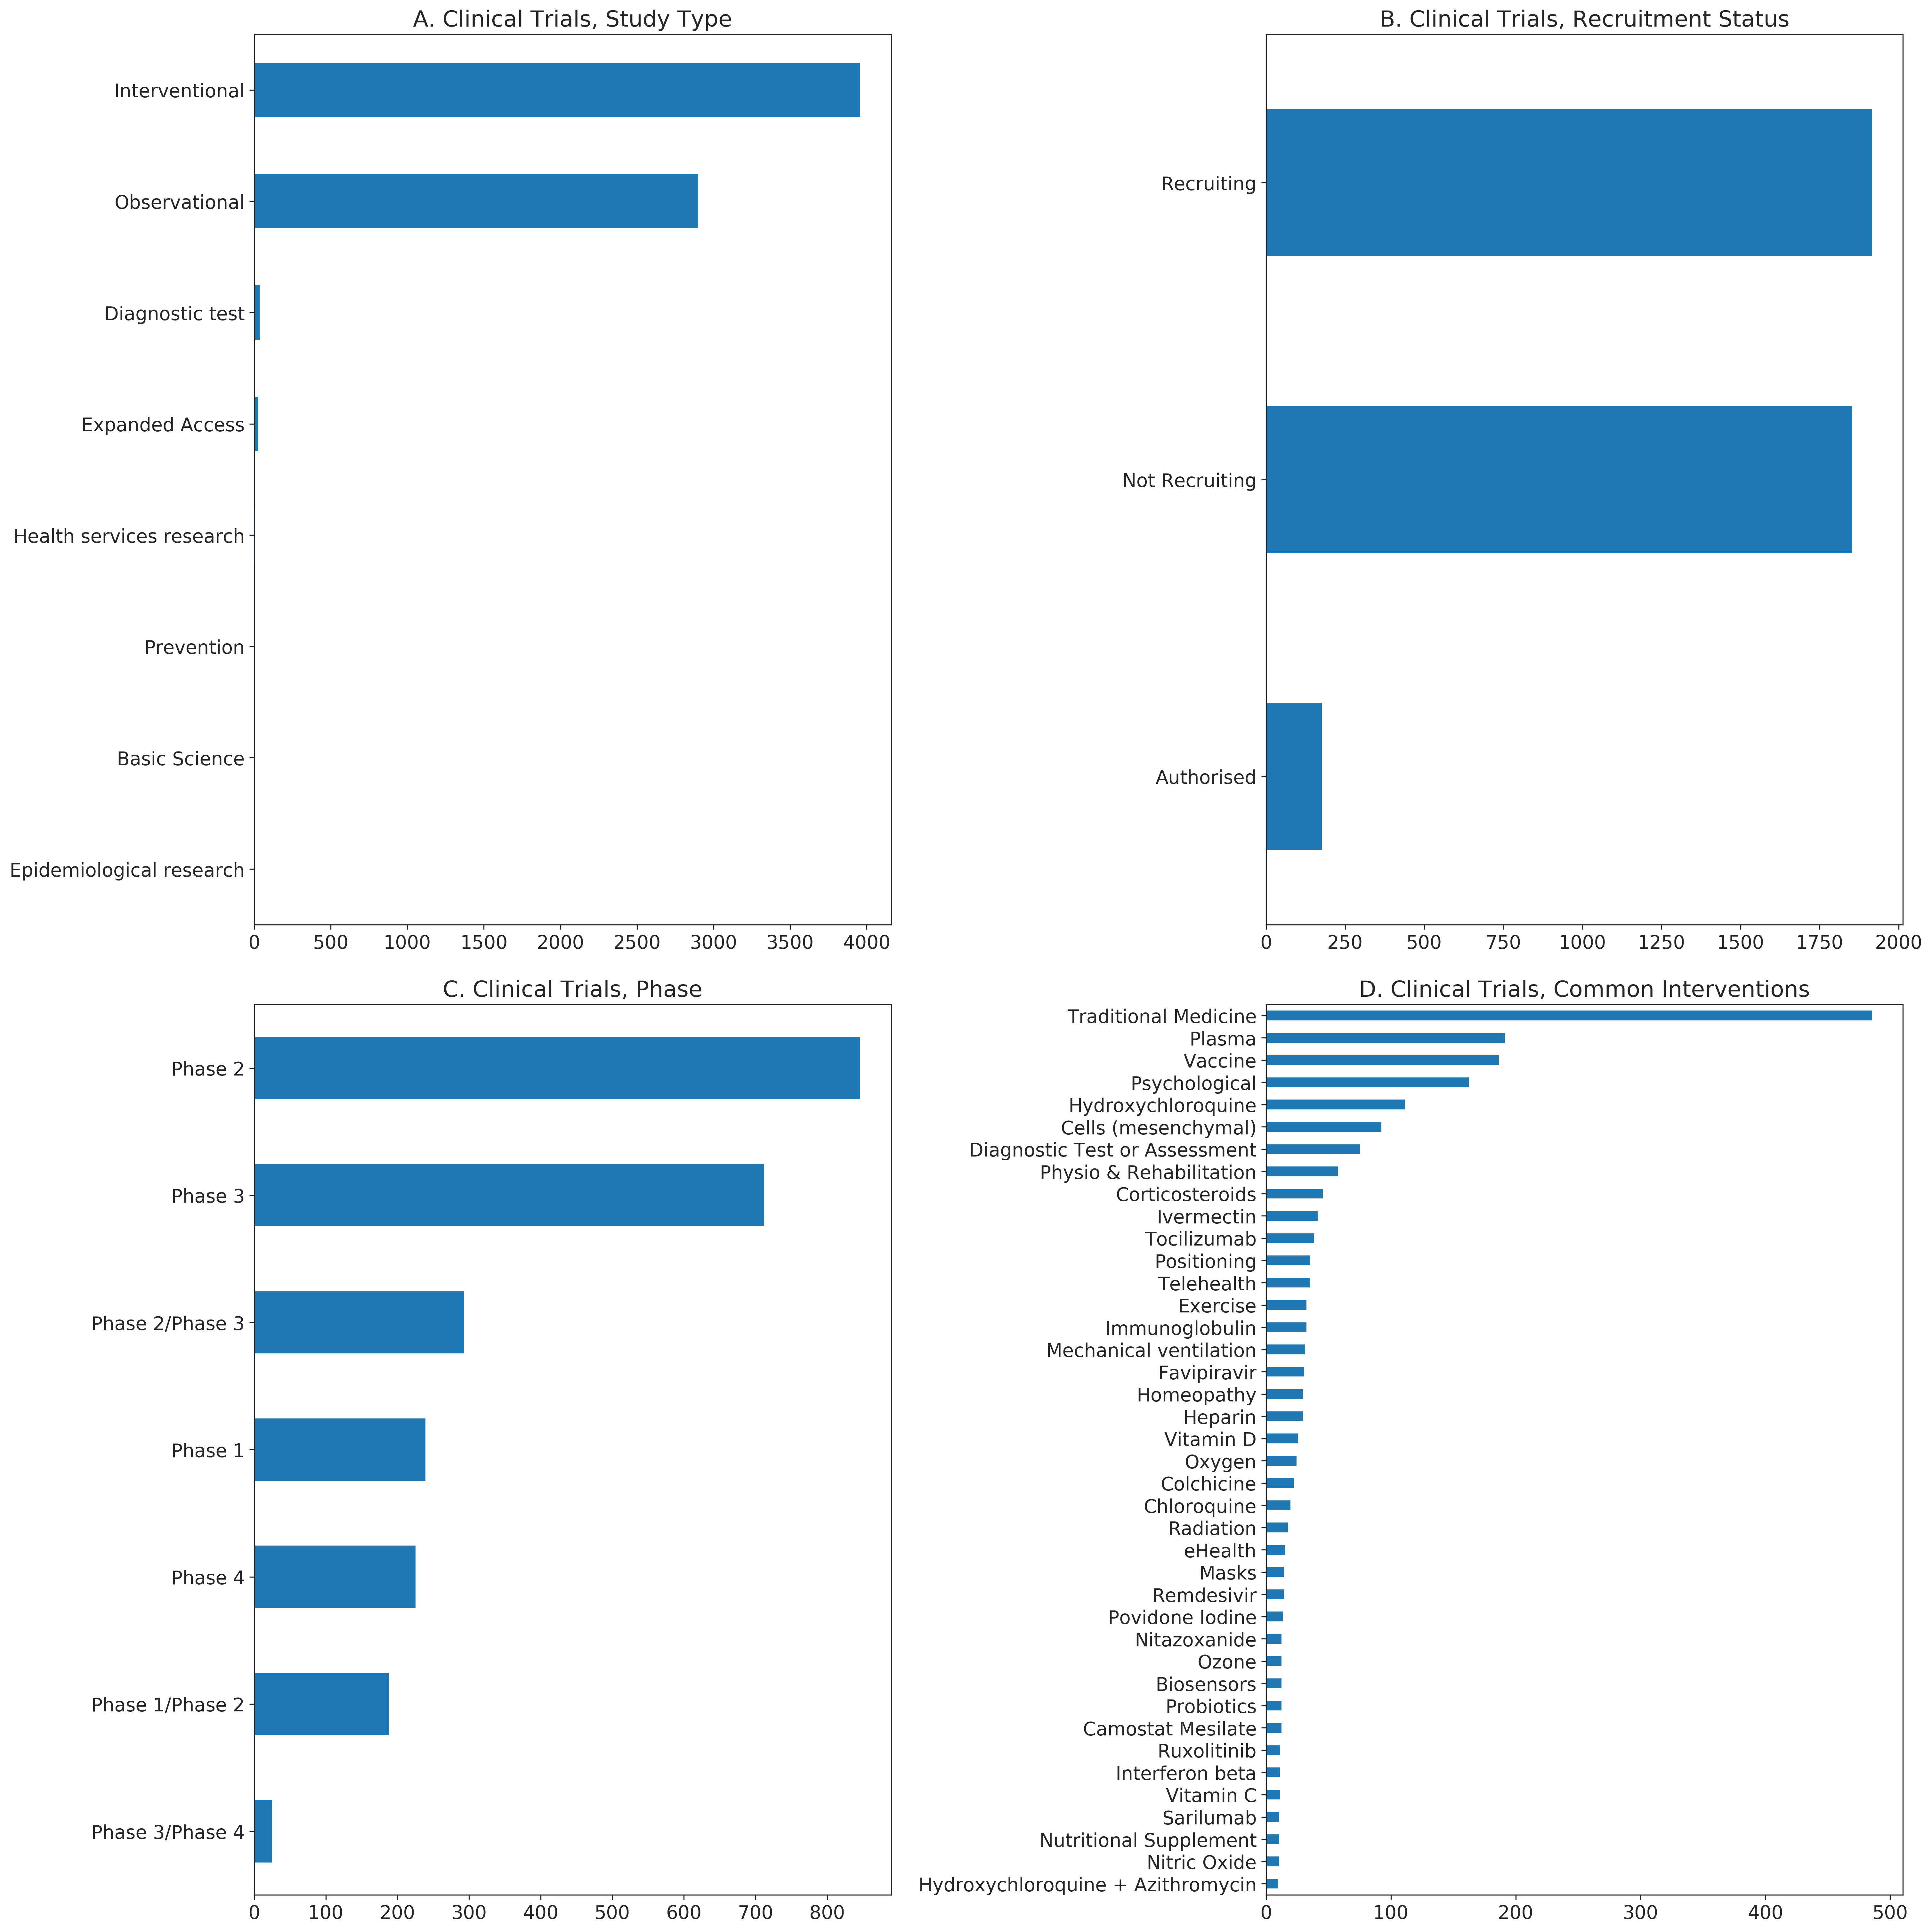
\includegraphics{(images/ebmdatalab-trials-original.png)https://github.com/greenelab/covid19-review/raw/e35e528aa516fc6177c057ee4c952cb6fc52cc5a/ebmdatalab/ebmdatalab-trials.png}
\caption{\textbf{Change in the COVID-19 clinical trials figure over time.}
When we first produced this figure on July 7, 2020, there were 3,733 clinial trials in the University of Oxford Evidence-Based Medicine Data Lab's COVID-19 TrialsTracker \citep{SSbnPnzT}.
As of November 9, 2020, it contains 6,417.
We were also able to easily reconfigure the figure prior to journal submission to emphasize interventional trials based on the recommendation of a collaborator who is a clinician.
This figure is included in an analysis of pharmaceutical development efforts during COVID-19 \citep{cifK9B8t}.}\label{fig:ebm-trials}
}
\end{figure}

Manubot's bibliographic management capabilities ended up being critical because the amount of relevant literature published far outstripped what we had anticipated at the beginning of the project.
As of April 30, 2021, there were 1,428 references (Figure \ref{fig:projectstats}).
The scite plugin provided a way to visually inspect the reference list to identify possible references of concern.
This and the other new features required for the COVID-19 project are now included in Manubot's rootstock, the template GitHub repository for creating a new manuscript.
Manubot and Zotero now support citing clinical trial identifiers such as \texttt{clinicaltrials:NCT04292899} \citep{yTCAmOyt}.
The scite integration and spell-checking functionalities have been integrated into the current release of Manubot.
Using CI, Manubot now checks that the manuscript was built correctly, runs spellchecking, and cross-references the manuscripts cited in this review.

\hypertarget{discussion}{%
\section{DISCUSSION}\label{discussion}}

The current project was managed through GitHub (https://github.com/greenelab/covid19-review) using Manubot \citep{YuJbg3zO} to continuously generate a version of the manuscript online \citep{yTsmmAYC}.
The Manubot framework facilitated a massive collaborative review on an urgent topic.
This project demonstrates that Manubot can be applied to projects where not all collaborators have expertise or even experience working with version control pipelines.
Through the development of cyberinfrastructure both for training novice users to interact with GitHub and to simplify the workflows to allow them to receive many of the benefits of What You See Is What You Get platforms such as Google Docs, we were able to adapt a powerful open publishing tool to harness the domain expertise of a large group of non-technical users and to respond to the flood of COVID-19 publications.

While Manubot manuscripts are written in markdown, they can be rendered in several formats that provide different advantages.
For example, beyond building just a PDF, Manubot also renders the manuscript in HTML, docx, and now, LaTeX.
The HTML manuscript format offers several advantages over a static PDF to harmonize available resources that we were able to apply to specific problems of COVID-19.
The integration of scite into the HTML build makes references more manageable by visually representing whether their results are contested or whether they have been corrected or retracted.
Cross-referencing different pieces of the manuscript, such as cited preprints with reviews stored in an appendix, is another dynamic option presented by HTML.
Additionally, because of the heavy emphasis on Word processing in biology, Manubot's ability to generate docx outputs was expanded to allow users to generate docx files containing only a section of the manuscript.
In our case, where the full project is nearly 100,000 words, this allows individual pieces to be shared widely.
Finally, the addition of LaTeX output is useful for researchers from computational fields who submit papers in tex format and removes the step of reformatting markdown prior to submission.

Working with biomedical scientists not only addressed the immediate goal of applying Manubot to the challenges of COVID-19, but also provided a second but equally important outcome.
Interested participants came from a wide range of backgrounds and many of the responses to the introductory issue emphasized a willingness to learn about a new topic, as well as an interest in COVID-19 and SARS-CoV-2 (Figure \ref{fig:wordcloud}).
``Biology'' was one of the most commonly emphasized interests, with almost double the number of uses as ``computational.''
This pattern suggests that, as anticipated, we primarily recruited researchers from traditional biological backgrounds.
The COVID-19 Review Consortium provided a platform for researchers to engage in scientific investigation during the initial phase of the COVID-19 pandemic during 2020 at a time when many biological scientists were unable to access their research spaces.
In turn, by seeking to adapt Manubot to allow for broader participation in open publishing from fields where computational training in tools like version control is uncommon, we made a number of improvements that are expected to increase its appeal to researchers from all backgrounds.
Manubot provided a way for all contributors, including ECRs, to join a massive collaborative project, demonstrating their individual contributions to the larger work and gaining experience with version control.
This project shows that massive online open publishing efforts can indeed advance scholarship through inclusion \citep{PoDz2q0A}, including during the extreme challenges presented by the COVID-19 pandemic.

\begin{figure}
\hypertarget{fig:wordcloud}{%
\centering
\includegraphics{images/interests.png}
\caption{\textbf{Visualization of collaborator interests as expressed in the introductory issue}
Potential collaborators were invited to practice commenting on an issue by sharing their academic backgrounds and interest in the project.
These responses were visualized using wordcloud2 in R (https://CRAN.R-project.org/package=wordcloud2).
Common responses included terms like contribute (44 uses), biology (42 uses), data (38 uses), help (36 uses), learn (32 uses), experience (31 uses), and student (25 uses).}\label{fig:wordcloud}
}
\end{figure}

With the worldwide scientific community uniting during 2020 and 2021 to investigate SARS-CoV-2 and COVID-19 from a wide range of perspectives, findings from many disciplines are relevant on a rapid timescale to a broad scientific audience.
As many other efforts have described, the publishing rate of formal manuscripts and preprints about COVID-19 has been unprecedented \citep{7ub6VM4Z}, and efforts to review the body of COVID-19 literature are faced with an ever-expanding corpus to evaluate.
In the case of the seven manuscripts produced by the COVID-19 Review Consortium, Manubot will allow for continuous updating of the manuscripts as the pandemic enters its second year and the landscape shifts with the emergence of promising therapeutics and vaccines \citep{cifK9B8t, i2CGFwI3}.
These manuscripts pull data from four data sources, allowing for information and visualizations to be updated daily using CI.
This computational approach allows for some of the updating process to be off-loaded so that domain experts can focus on the broader implications of new information as it emerges.
As a result, centralizing, summarizing, and critiquing data and literature broadly relevant to COVID-19 can help to expedite the interdisciplinary scientific process that is currently happening at an advanced pace.
The efforts of the COVID-19 Review Consortium illustrate the value of including open source tools, including those focused on open publishing, in these efforts.
By facilitating the versioning of text, such platforms also allow for documentation of the evolution of thought in an evolving area.
This application of version control holds the potential to improve scientific publishing in a range of disciplines, including those outside of traditional computational fields.
While Manubot is a technologically complex tool, this project demonstrates that it can be broadly appealing even outside of technical and/or computational areas of research.

\hypertarget{acknowledgements}{%
\section*{Acknowledgements}\label{acknowledgements}}
\addcontentsline{toc}{section}{Acknowledgements}

We are grateful to Josh Nicholson and Milo Mordaunt for their support with the scite plugin, and to David Nicholson for the suggestion and feedback to enable the reporting of the locations of spelling errors in the spell-checker tool.
We thank Nick DeVito for assistance with the Evidence-Based Medicine Data Lab COVID-19 TrialsTracker data.


	\balance
	\bibliography{methods.bib}

\end{document}
\endinput
%%
%% End of file `sample-authordraft.tex'.
